% document formatting
\documentclass[10pt]{article}
\usepackage[utf8]{inputenc}
\usepackage[left=1in,right=1in,top=1in,bottom=1in]{geometry}
\usepackage[T1]{fontenc}
\usepackage{xcolor}

% math symbols, etc.
\usepackage{amsmath, amsfonts, amssymb, amsthm}

% lists
\usepackage{enumerate}

% images
\usepackage{graphicx} % for images

% code blocks
\usepackage{minted, listings} 

% verbatim greek
\usepackage{alphabeta}

\graphicspath{{./assets/images}}

\newcommand{\solution}{\textbf{Solution:}} 
\newcommand{\example}{\textbf{Example: }}

\title{EC ENGR 102 Week 1}

\author{Aidan Jan}
\date{\today}

\begin{document}
\maketitle
\section*{Introduction}
\begin{itemize}
    \item Society relies on being able to:
    \begin{enumerate}
        \item Represent information (Signals)
        \item Communicate, process, and operate on that information (Systems)
    \end{enumerate}
    \item Technology is a reflection of our ability to do these things.
\end{itemize}
The Signals and Systems perspetive is basically:
\begin{itemize}
    \item Information is represented as "signals", and information changes, or is processed, through "systems".
\end{itemize}
\subsection*{Examples of signals and systems}
\begin{itemize}
    \item My voice is a \textbf{signal}, and my cell phone (\textbf{a system}) records it, transforms it into a transmittable form, communicates it to a cell phone tower(s), eventually reaching the person I'm speaking to who hears it... in almost real time.
    \item YouTube videos are a \textbf{signal}, and our computer or phone (\textbf{a system}) plays them, adjusting their resolution based on our WiFi speed, etc.
    \item Moving a computer mouse or typing on a keyboard is a \textbf{signal}, and our computer then uses circuits (\textbf{a system}) to translate this information to show you an updated computer screen.
    \item Note that signals and systems \textbf{are not} limited to digital signals.
    \begin{itemize}
        \item Any physical or abstract quantity that can be measured is a \textbf{signal}.
        \begin{itemize}
            \item The federal deficit is a \textbf{signal}\dots
        \end{itemize}
        \item Anything that changes a signal is a \textbf{system}
        \begin{itemize}
            \item Policies passed by Congress, the interaction of national and global economies, etc. are \textbf{systems}.
        \end{itemize}
        \item This is a general abstraction.
    \end{itemize}    
\end{itemize}
\textbf{The goal of the signals and systems abstraction is to decompose a problem into components with the following block diagram.}
\[\text{Input signal } x(t) \longrightarrow \boxed{\text{System}} \longrightarrow \text{ Output signal }y(t)\]
This abstraction enables systems can be combined together to form composite systems.
\subsection*{A Diversity of Signals and Systems}
How do we (rigorously) represent signals and systems, considering their variety?
\begin{itemize}
    \item The short answer: depending on the application, there can be several ways to represent signals; \textbf{how we represent signals, and what we aim to do with them, determines the types of tools we need to analyze them.}
    \item In traditional signal processing, signals are 1-D, and do not have a noise model.  Ex. Radio, communications, control systems, circuit analysis.
    \item In statistical signal processing, signals can be multi-dimensional, and incorporate noise models.  Ex. Communications over noisy channels, information theory, noisy control.
    \item In machine learning: signals can be multi-dimensional, and incorporate noise models.  Ex. AI, neural networks and deep learning, prediction systems, unsupervised learning.
    \item This class will focus on traditional signal processing.
\end{itemize}
\subsection*{Signals in ECE 102}
What is a signal?
\begin{itemize}
    \item A signal is a \textit{function} of one or more variables
    \item What is a function?
    \begin{itemize}
        \item We ought be familiar with functions from mathematics: denoted by $f(\cdot)$, it typically accepts some input, $x$ and return some output, $y$.  We write this as:
        \[y = f(x)\]\
        \item We usually denote this function as: $f \::\: \mathbb{R} \rightarrow \mathbb{R}$, indicating that $f$ is a function mapping a real number (the first $\mathbb{R}$) to another real number (the second $\mathbb{R}$).
    \end{itemize}
\end{itemize}
\subsubsection*{The Time Domain}
Signals usually have to do with \textit{time} domain representations
\begin{itemize}
    \item That is, signals are usually functions that accept an input time $t$, and return the value of the signal at that time.  For example, a signal could be represented $x(t)$, which denotes the value of the signal at time $t$.
\end{itemize}
\subsubsection*{Music}
\begin{itemize}
    \item Suppose you recorded your voice or a musical instrument.  Your computer (system) recorded a sound (signal), which can be mathematically modeled as a sine wave.
    \item When you hear it, played out from your speaker, the sound wave (signal) vibrates bones located inside your ear (system), which vibrates hair cells present, which transmits the neural signal to your brain.
    \item Music is essentially a combined sine wave.
\end{itemize}
\textbf{Aside: One of the great secrets of the Universe}
\begin{itemize}
    \item "Every signal has a spectrum and is determined by its spectrum.  You can analyze the signal either in the time (or spatial) domain or in the frequency domain.  I think this qualifies as a Major Secret of the Universe."  -Prof. Brad Osgood, Stanford University.
    \item A "spectrum" is basically a graph where frequency is on the x-axis, and power on the y-axis.  Instead of a Concert A being represented as a sine wave at 440 Hz., it can be represented by its spectrum, which is a graph with a peak at the 440Hz. frequency.  (Basically, run FFT on the signal to get the spectrum.)
\end{itemize}
\example
\begin{center}
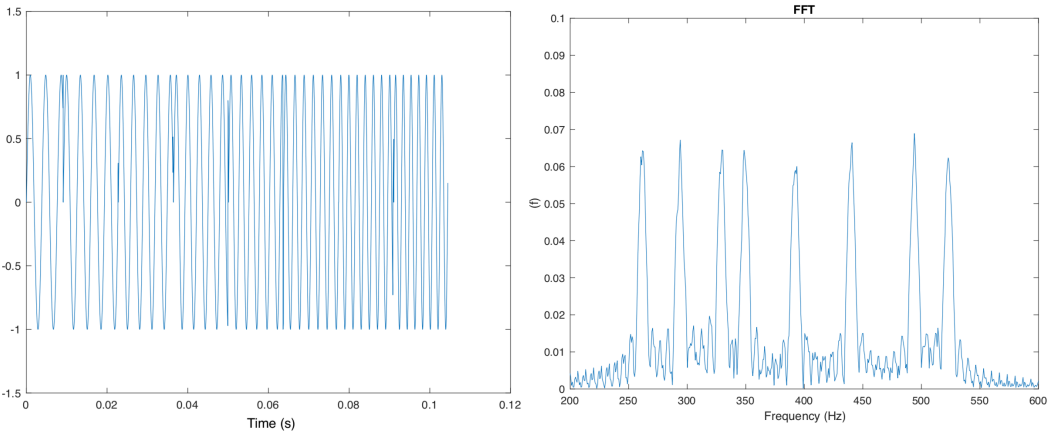
\includegraphics[scale=0.7]{W1_1.png}\\
Left: Sine wave of sound signal.  Right: Spectrum of sound signal (FFT)
\end{center}
Notice that the spectrum generated does not display time!  By observing the peaks on the left sine wave, we can tell it is an ascending scale, but the spectrum does not show that!\\\\
\example
\begin{center}
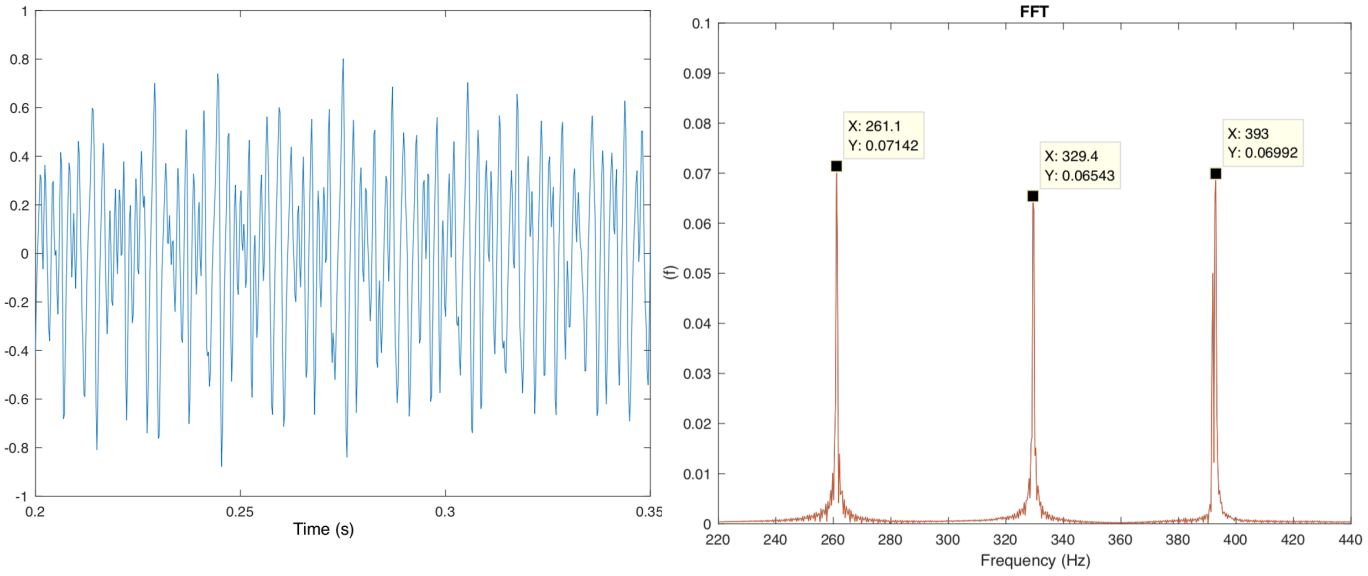
\includegraphics[scale=0.6]{W1_2.png}\\
This is the waveform and spectrum of the C-Major Triad.  The transform (a function) can bring context to a seemingly unintelligible waveform.
\end{center}
\begin{itemize}
    \item We can run functions in the spectrum domain!  Say for example we want to recover the C from the triad waveform.  This would be incredibly difficult to do in the waveform graph, but easy in the spectrum graph.  All we have to do is to set a filter.  For example, our filter can multiply all the frequencies above 300Hz by zero.  Then, convert the remaining frequencies back to a waveform.
\end{itemize}
\subsection*{Sine waves are important}
\begin{itemize}
    \item When we talk about music, we talk about sine waves with frequencies of units \textbf{Hertz}.
    \item Radio frequencies, wireless communication, music, etc.  It would not be an exaggeration to say that none of this technology would exist without the math that we'll learn in ECE 102.  
    \item Any signal can be formed by adding sine waves.
    \item \textbf{The Bottom Line:} once we understand the mathematics of how to create things with sine waves (frequency domain or spectrum), we can do very powerful operations.  This is the basis for many technologies that we may (sometimes) take for granted.
\end{itemize}
\subsection*{Applications of Signals and Systems}
\begin{itemize}
    \item The design of analog circuits
    \item Magnetic resonance imaging (MRI)
    \item Traditional control systems
    \item Mixing music
\end{itemize}

\section*{Signals}
\subsection*{Discrete vs. Continuous Signals}
\begin{itemize}
    \item A continuous signal is one that is defined for every point in time.
    \item A discrete signal is one that is defined at individual points
    \item Continous signals can be graphed as lines, discrete signals are graphed as points.
\end{itemize}
\subsection*{Signal Operations}
\subsubsection*{1. Amplitude Scaling}
Suppose we have a signal $x(t) = \alpha\sin(t)$.
\begin{itemize}
    \item If we choose a value of $\alpha$ that is between 0 and 1, the signal gets smaller. (\textit{attenuation})
    \item If $\alpha$ is greater than 1, the signal is amplified. (\textit{amplification})
    \item If $\alpha$ is negative, the signal is flipped.  (\textit{inversion})
\end{itemize}
\subsubsection*{2. Time Scaling}
Suppose we have a signal $x(t) = \sin(\alpha t)$.
\begin{itemize}
    \item If the value of $\alpha$ is between 0 and 1, the signal's period increases.  (\textit{Time expansion})
    \item If the value of $\alpha$ is greater than 1, the signal's period decreases.  (\textit{Time compression})
    \item If the value of $\alpha$ is less than 0, the time of the signal is reversed.  (\textit{Time reversal})
\end{itemize}
\subsubsection*{3. Time Shift}
Suppose we have a signal $x(t) = \sin(t - \alpha)$
\begin{itemize}
    \item If $\alpha$ is positive (e.g., you are subtracting a positive number), the signal is delayed.  (\textit{Delayed signal})
    \item If $\alpha$ is negative (e.g., you are subtracting a negative number), the signal is advanced. (\textit{Advanced signal})
\end{itemize}
\subsection*{Combining Operations}
Suppose we have a function that is zero everywhere, except between -1 and 1, where the function evaluates to 1.  Let $x(t)$ represent this function.
\textbf{What is $x(2(t - 1))$?}\\\\
The naive method (\textbf{Incorrect}):
\begin{itemize}
    \item First, apply the time delay.  Now the signal is 1 between $x=0$ and $x=2$.
    \item Next, apply the compression by a factor of 2.  Now the signal goes from $x=0$ to $x=1$.
    \item The result is a signal that is zero everywhere, but is 1 between $x = 0$ and $x = 1$.
\end{itemize}
The above answer is incorrect.  Why?
\begin{itemize}
    \item We can test this with $x(1)$, which should evaluate to 1.
    \item To make $x(2(t - 1))$ equivalent to $x(1)$, we set $t = 1.5$.  In our proposed answer, $t = 1.5$ results in 0, where it should result in $1$, matching the original.
\end{itemize}
The correct method:
\begin{itemize}
    \item Do reverse PEMDAS -> SADMEP.
    \item First, apply the time compression.  (Instead of the parenthesis, time delay first)  Now the signal begins at $t = -0.5$ and ends at $t = 0.5$.
    \item Now, we apply the time delay.  Now the signal begins at $t = 0.5$ and ends at $t = 1.5$.
    \item This gives the correct result. 
\end{itemize}
Alternatively, simply distribute the 2 into the parenthesis and separate all the terms.  That would also fix the problem.
\subsection*{Even and Odd Decomposition}
\begin{itemize}
    \item An even function is a $f(x)$ such that $f(-x)$ = $f(x)$.
    \item An odd function is a $f(x)$ such that $f(-x)$ = $-f(x)$.
\end{itemize}
Suppose we have the following function:
\begin{center}
    
\includegraphics[scale=1]{W1_3.png}
\end{center}
Let's make an assertion that $x(t) = x_e(t) + x_o(t)$, where $x_e$ is some even function and $x_o$ is some odd function.  How do we find the functions?\\\\
Our goal is to define $x_e(t)$ and $x_o(t)$ in terms of $x(t)$.\\
First, let's rearrange the equation
\[x_e(t) = x(t) - x_o(t)\]
\[x_o(t) = x(t) - x_e(t)\]
Following the rules of odd functions, we can do
\[x_o(t) = -(x(-t) - x_e(-t))\]
Simplifying the even function, we get 
\[x_o(t) = -(-x(-t) - x_e(t))\]
\[x_o(t) = x(-t) + x_e(t)\]
Plugging this for $x_o(t)$ in the first equation, we get
\[x_e(t) = x(t) + x(-t) - x_e(t)\]
\[\boxed{x_e(t) = \frac{1}{2}\left(x(t) + x(-t)\right)}\]
The odd function can be found by rearranging the original even function, then plugging it into the odd function.
\subsection*{Periodic Signals}
\begin{itemize}
    \item The concept of periodic signals is very important in this class.  Colloquially, these are signals that repeat after a given interval, $T_0$.
    \item The formal definition of a periodic signal is as follows:
    \begin{itemize}
        \item A continuous time signal is periodic if and only if there exists a $T_0 > 0$ such that
        \[x(t + T_0) = x(t)\]
            for all $t$.  $T_0$ is called the period of $x(t)$.
    \end{itemize}
\end{itemize}
\subsubsection*{Periodic signal properties}
Suppose $x(t)$ is periodic.
\begin{align*}
    x(t + T_0) &= x(t)\\
    x(t + 2 \cdot T_0) &= x(t)\\
    &= x(t + T_0 + T_0)
\end{align*}
Define $\tau = t + T_0$.  By substitution,
\begin{align*}
    x(t + 2 \cdot T_0) &= x(\tau)\\
    &= x(t + T_0)
\end{align*}
Therefore, $x(t + nT_0) = x(t)$ is true, where $x(t)$ is periodic, for all integers $n$.\\
The smallest $T_0$ for which $x(t + T_0) = x(t)$ is called the \textbf{"fundamental period"}.

\subsubsection*{Sinusoids}
The most basic signal in this class is the sine or consine wave.  We'll use them \textit{extensively} so it's worth reviewing their properties.  By the end of this class, you'll be proficient at manupulating sinusoids.\\
A cosine function is defined by:
\begin{align*}
    x(t) &= A \cos(\omega t - \theta) \\
    &= A \cos(2\pi ft - \theta)
\end{align*}
\begin{itemize}
    \item $\omega = 2 \pi f$, and represents \textit{angular frequency}.
    \item $f$ represents frequency, and is measured in Hertz.  $f = \frac{1}{T_0}$
\end{itemize}

\subsection*{Rules from trigonometry}
Some additional properties that you should be familiar:
\begin{itemize}
    \item $\sin(\theta) = \cos(\theta - \frac{\pi}{2})$
    \item $\cos$ is even and $\sin$ is odd
    \item $\frac{d}{dt} \sin(\theta) = \cos(\theta)$ and $\frac{d}{dt}\cos(\theta) = -\sin(\theta)$
    \item $\sin^2(\theta) + \cos^2(\theta) = 1$
    \item Suppose we have the sum or product of two periodic signals.  Let $x_1$ be the period $T_1$ and $x_2$ be the period $T_2$.  If $x_1$ and $x_2$ share a \textbf{integer} common multiple, then the resulting function is also periodic.
    \begin{itemize}
        \item If the period of $f(t)$ is 4 and the period of $g(t)$ is 5, then the resulting sum or product, $f(t) + g(t)$ or $f(t) \cdot g(t)$ would have a period of 20.
        \item If the period of $f(t)$ is 4 and the period of $g(t)$ is $\pi$, then the resulting sum or product is not periodic.
    \end{itemize}
\end{itemize}

\subsection*{Periodic Extension}
In this class, we will sometimes be interested in taking an aperiodic signal and making its periodic extension.  What this means is that we take some interval on this signal of length $T_0$ and repeat it, as illustrated below:
\begin{center}
    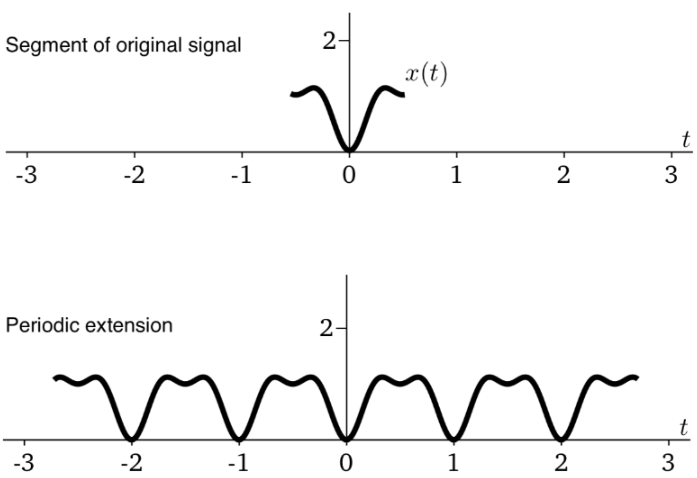
\includegraphics[scale=0.8]{W1_4.png}
\end{center}

\subsection*{Causality}
Another signal property is the concept of causality.  It is important to define causality because in real life, we typically can only work with signals in the present and past (i.e., we don't know the future).  This will become more clear when we discuss convolution and filtering.
\begin{itemize}
    \item Causal signals are non-zero only for $t \geq 0$.  Colloquially, the signal starts at $t = 0$ or later.
    \item Noncausal signals are non-zero for some $t < 0$.  Colloquially, the signal starts before $t = 0$.
    \item Anticausal signals are non-zero only for $t \leq 0$.  Colloquially, these signals only exist before $t = 0$ and typically are interpreted as running backwards in time.
\end{itemize}

\subsection*{Signal Energy and Power}
We know from circuits that the voltage signal, $v(t)$, and current signal, $i(t)$, across a resistor, $R$ is related through:
\[v(t) = i(t)R\]
and further, that the signal's instantaneous power at time $t$ is:
\[p(t) = v(t)i(t)\]
If we consider that $R = 1 \Omega$, then we see that
\begin{center}
    \begin{align*}
        p(t) &= v^2(t) \\
        &= i^2(t)
    \end{align*}
\end{center}
This is to show that power is proportional to the signal quantity squared; if resistance was not 1, it would only scale power by a constant.  In most cases, this is not \textit{actual power} in that most signals aren't applied to a $1 \Omega$ resistor.\\\\
Signal power has units of Watts (Joules per time).  Hence, to get the total energy of a signal, $x(t)$, across all time, we integrate the power.
\[\boxed{E_x = \lim_{T \rightarrow \infty} \int_{-T}^T \vert x(t) \vert^2 \:\text{d}t}\]
(We incorporate the absolute value, $\vert \cdot \vert$, in case $x(t)$ is a complex signal.)  Like signal power, signal energy is usually not an \textit{actual} energy.\\\\
We can also caltulate \textit{average power} of the signal by calculating:
\[\boxed{P_x = \lim_{T \rightarrow \infty} \frac{1}{2T} \int_{-T}^T \vert x(t) \vert^2 \:\text{d}t}\]
\begin{itemize}
    \item If $0 < E < \infty$, $x(t)$ is called an "\textit{energy signal}"
    \item If $0 < P < \infty$, $x(t)$ is called a "\textit{power signal}"
\end{itemize}
~\\
\example
\begin{itemize}
    \item $x(t) = e^{-t^2}$ is an energy signal, for its integral from negative to positive infinity converges to a finite number.  In this case, $\sqrt{\pi}$.
    \begin{itemize}
        \item Energy signal means there is a finite amount of power in total, from the beginning to end of time.
        \item If $\vert x(t) \vert^2 \propto \frac{1}{t^2} \rightarrow$ energy signal
        \item If $\vert x(t) \vert^2 \propto \frac{1}{\sqrt{t}} \rightarrow$ not an energy signal
        \item The border is $\frac{1}{t}$.  If it decays faster, it is an energy signal.  Otherwise, it is not.
        \item Every energy signal \textbf{has 0 power} since a finite amount of energy distributed over an infinite amount of time converges to 0.
    \end{itemize}
    \item $x(t) = \cos(\omega t)$ is a power signal.
    \begin{itemize}
        \item $\vert x(t)\vert^2 = \cos^2(\omega t)$, which there exists a constant finite average power.
        \item For a periodic signal, the way to find the average power easily is to calculate the average power for one period.
        \item Every power signal \textbf{has infinite energy} since a finite amount of energy times an infinite amount of time diverges to infinity.
    \end{itemize}
    \item A signal cannot be both an energy signal and a power signal.  However, there can be signals that are neither energy nor power.
\end{itemize}
~\\
\example
\[x(t) = a \cdot \sin(\omega_0 t)\]
This is a power signal because it is periodic; there isn't a finite amount of energy.
\begin{itemize}
    \item $E_x = \infty$
    \item $P_x = \frac{a^2}{2}$
\end{itemize}
\example
\[x(t) = \begin{cases} Ae^{-at} & t \geq 0, a > 0 \\ 0 & \text{else}\end{cases}\]
\begin{itemize}
    \item $P_x = 0$
    \item $E_x = \frac{A^2}{2a}$\\
\end{itemize}
Sanity check:
\begin{align*}
E_x &= \int_{-\infty}^{0} 0 \cdot \text{d}t + \int_0^\infty (Ae^{-at})^2 \:\text{d}t\\
&= \int_0^\infty A^2 e^{-2at} \:\text{d}t\\
&= \frac{A^2}{-2a}\bigg\vert_{t = 0}^{t = \infty}\\
&= 0 - \left(-\frac{A^2}{2a}\right)\\
&= E_x = \frac{A^2}{2a}
\end{align*}

\subsection*{Complex Sinusoids}
So far, all signals we've presented are real-valued.  But signals can also be complex.
\begin{itemize}
    \item A complex signal is one that takes the form:
    \[z(t) = x(t) + jy(t)\]
    where $x(t)$ and $y(t)$ are real-valued signals and $j = \sqrt{-1}$
    \item $j$ is used instead of $i$ because electrical engineers use $i$ for current.
\end{itemize}
\subsubsection*{Review of complex numbers}
\begin{itemize}
    \item A complex number is formed from two real numbers, $x$ and $y$, via:
    \[z = x + jy\]
    why $j = \sqrt{-1}$.  Hence, a complex number is simply an ordered pair of real numbers, $(x, y)$.
    \item $x = \mathfrak{R}(z)$ is called the \textit{real} part of $z$.  In this class we will also write $x = \text{Re}(z)$.
    \item $y = \mathfrak{I}(z)$ is called the \textit{imaginary} part of $z$.  In this class we will also write $y = \text{Im}(z)$.
\end{itemize}
\subsubsection*{Polar Representation of Complex Numbers}
The same complex number can be written in polar form,
\begin{align*}
    z &= x + jy\\
    &= re^{j \phi}
\end{align*}
where 
\begin{itemize}
    \item $r$ is the \textit{modulus} or \textit{magnitude} of $z$.
    \item $\phi$ is the \textit{angle} or \textit{phase} of $z$.
    \item $e^{j\phi} = \cos(\phi) + j\sin(\phi)$.  We will sometimes write this as $\exp(j\phi)$.
\end{itemize}
\begin{center}
    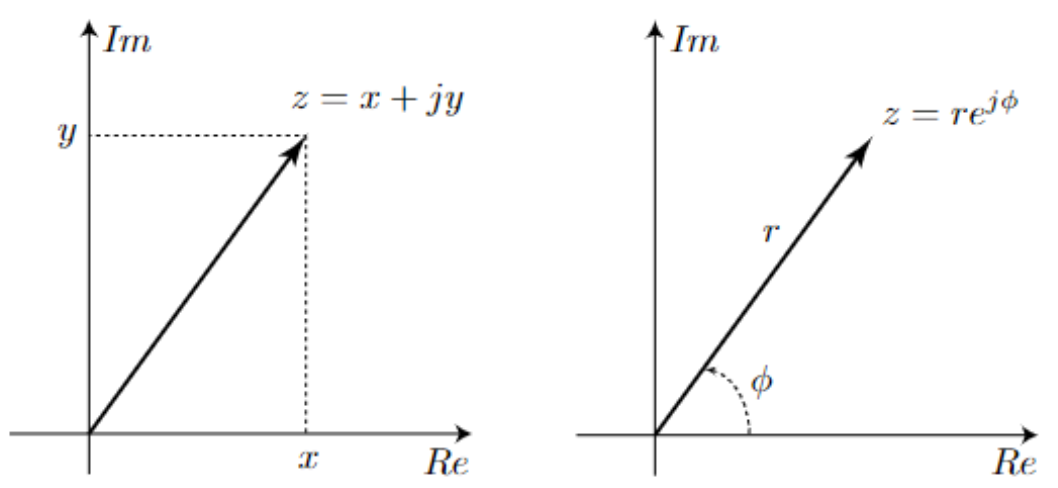
\includegraphics[scale=0.6]{W1_5.png}
\end{center}
Here are the same intuitions from Cartesian and polar coordinates hold.
\begin{itemize}
    \item $x = r \cos(\phi)$
    \item $y = r\sin(\phi)$
    \item $r = \sqrt{x^2 + y^2}$
    \item $\phi = \arctan\left(\frac{y}{x}\right)$
\end{itemize}
\subsubsection*{Complex relations}
Here are a few relations:
\begin{itemize}
    \item \textbf{Complex conjugate:} If $z = x + jy$, then $z^*$, the complex conjugate of $z$,
    \[z^* = x - jy\]
    \item \textbf{Modulus and complex conjugate.}  The following relation holds:
    \[\vert z \vert^2 = z^*z = zz^*\]
    This is because
    \begin{align*}
        zz^* &= (x + jy)(x - jy) \\
        &= x^2 + y^2\\
        &= r^2
    \end{align*}
    where $r = \sqrt{x^2 + y^2}$ as described above.
    \item \textbf{Inverse of $j$.}  Since $j^2 = -1$, we have that $-j = \frac{1}{j}$.
\end{itemize}

\subsubsection*{Example using Euler's Formula}
\begin{align*}
    \cos(\theta) &= \frac{1}{2} \left(e^{j\theta} + e^{-j \theta}\right)\\
    \sin(\theta) &= \frac{1}{2j} \left(e^{j\theta} - e^{-j \theta}\right)
\end{align*}
Using these, you can very easily derive the Law of Cosines.

\subsection*{Signal Models}
\subsubsection*{Sinusoids}
We have all seen real sinusoids.
\[x(t) = A \cos(\omega t - \theta)\]
Now \dots there are complex sinusoids.\\\\
The complex sinusoid is given by:
\[Ae^{j(\omega t + \theta)} = A \cos(\omega t + \theta) + jA \sin(\omega t + \theta)\]
We draw complex signals with dotted lines.
\begin{center}
    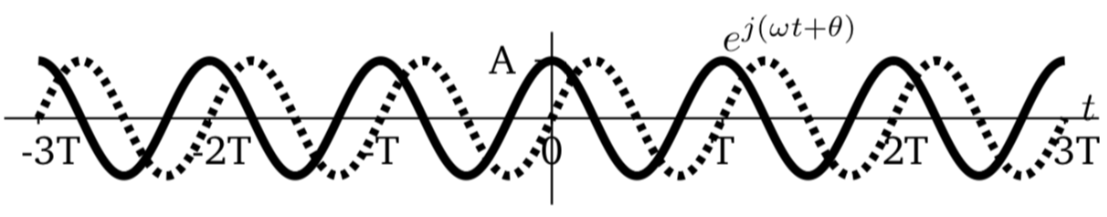
\includegraphics[scale=0.6]{W1_6.png}
\end{center}
The real part of the complex sinusoid (solid line) is:
\[\mathfrak{R}\left(Ae^{j(\omega t + \theta)}\right) = A \cos(\omega t + \theta)\]
The imaginary part of the complex sinusoid (dotted line) is:
\[\mathfrak{I}\left(A e^{j(\omega t + \theta)}\right) = A \sin(\omega t + \theta)\]

\subsubsection*{Exponential Signals}
An exponential signal is given by
\[x(t) = e^{\sigma t}\]
\begin{itemize}
    \item If $\sigma > 0$, this signal grows with increasing $t$ (black signal in the plot below).  This is called exponential growth.
    \item If $\sigma < 0$, this signal decays with increasing $t$ (blue signal in the plot below).  This is called exponential decay.
\end{itemize}
\begin{center}
    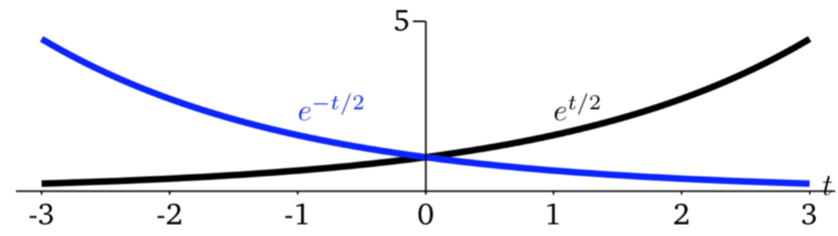
\includegraphics[scale=0.6]{W1_7.png}
\end{center}

\subsubsection*{Damped or Growing Sinusoids}
A damped or growing sinusoid is denoted
\[x(t) = e^{\sigma t} \cos(\omega t + \theta)\]
The sinusoid will grow exponentially if $\sigma > 0$ and decay exponentially if $\sigma < 0$.
\begin{center}
    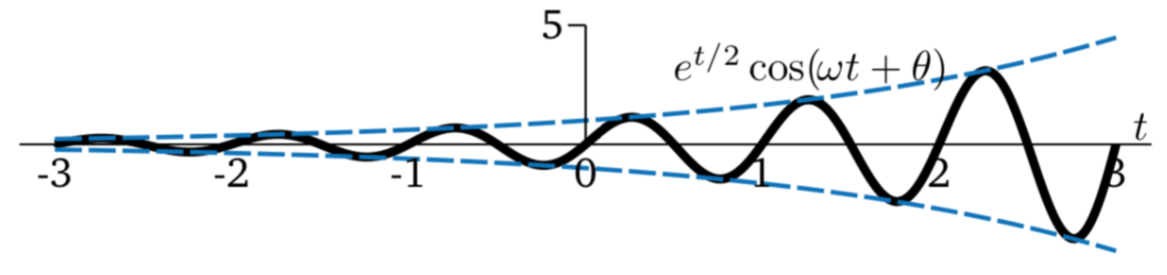
\includegraphics[scale=0.6]{W1_8.png}
\end{center}
There are also complex exponentials!  They are denoted:
\[x(t) = e^{(\sigma + j\omega)}t\]
It is a combination of the complex sinusoid and an exponential.  All prior signals are special cases of the complex exponential signal.
\begin{center}
    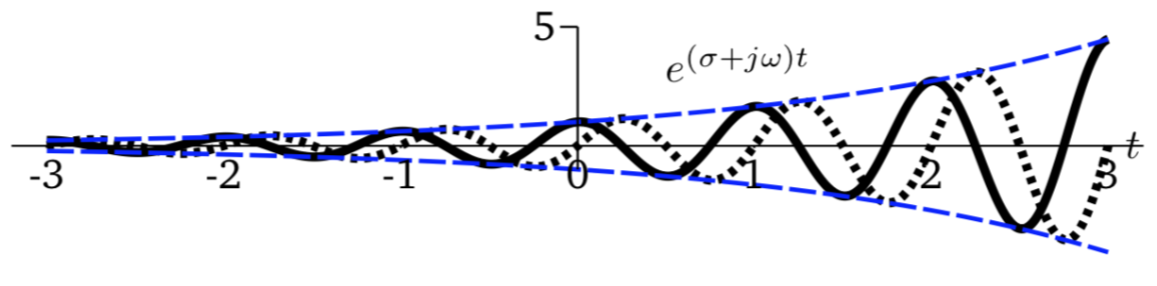
\includegraphics[scale=0.6]{W1_9.png}
\end{center}
It is helpful to think of $\sigma$ and $j\omega$ in the complex plane.  $\sigma$ is the x-axis and $j\omega$ is the y-axis.  Then complex exponentials in the left complex plane are decreasing signals and those in the right are increasing signals.
\begin{itemize}
    \item Basically, you can define any complex exponential using two points in the complex plane, $\sigma$ and $j\omega$.
\end{itemize}
\begin{center}
    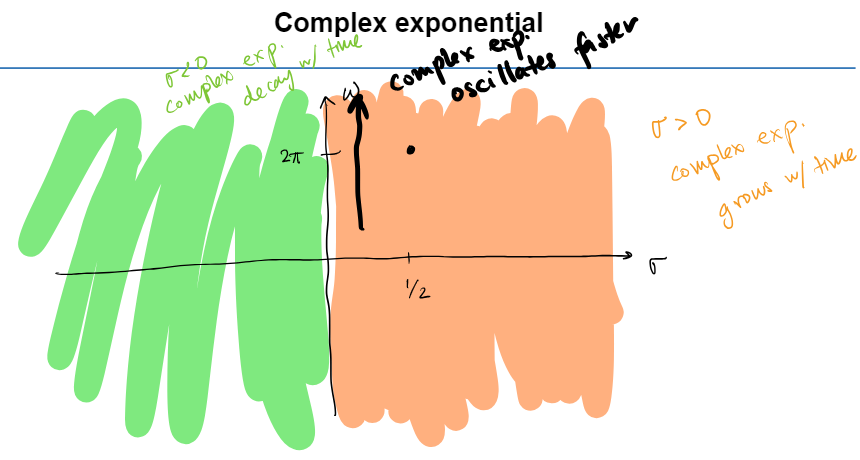
\includegraphics[scale=0.8]{W1_10.png}
\end{center}
\end{document}
